\documentclass[11pt,a4paper,landscape]{article}
\usepackage[margin=1.3cm]{geometry}
\usepackage{tikz}
\usetikzlibrary{arrows.meta}
\pagestyle{empty}
\renewcommand{\familydefault}{\sfdefault}
\hyphenpenalty=10000
\exhyphenpenalty=10000
\begin{document}
\begin{center}
{\Large\bfseries Round 3: lifecycle memory and role-specific actor--critic}\par
\vspace{2mm}
{\small Student 26510121 \quad | \quad Implemented modules, not a claim of optimality}
\vspace{4mm}

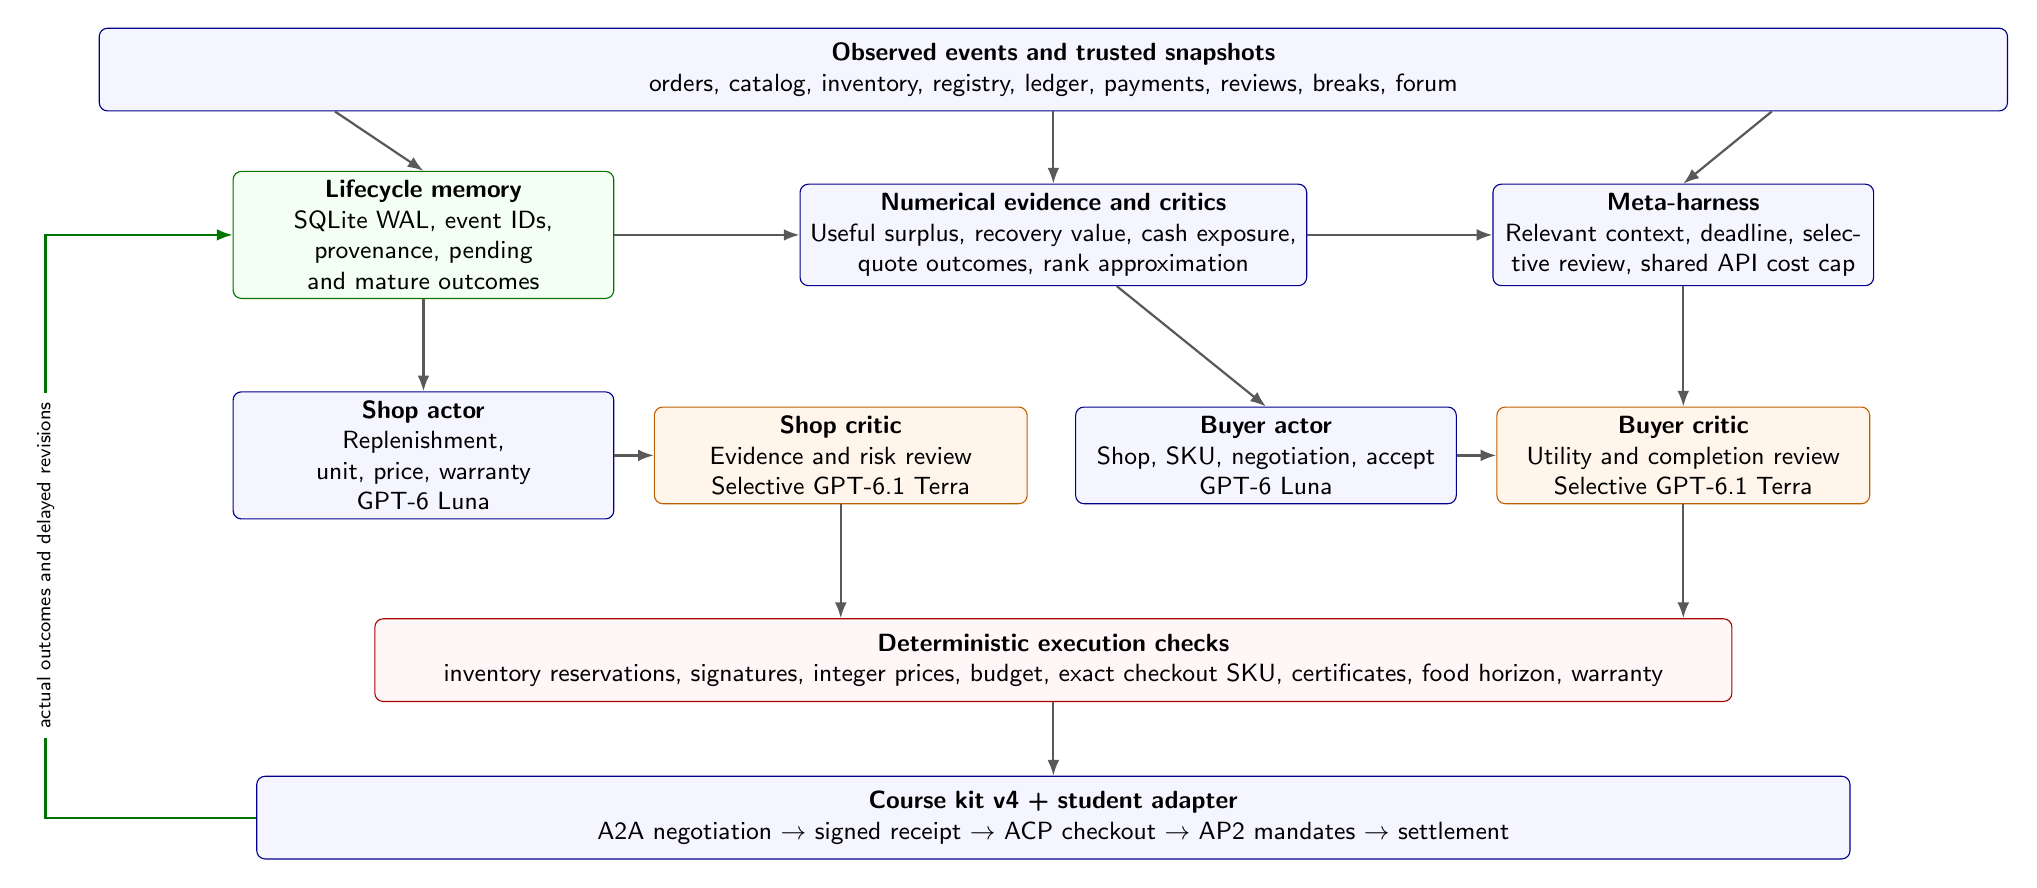
\begin{tikzpicture}[
  box/.style={draw=blue!55!black,fill=blue!4,rounded corners=3pt,align=center,
              text width=4.6cm,minimum height=1.05cm,font=\small},
  critic/.style={box,draw=orange!75!black,fill=orange!8,text width=4.5cm},
  flow/.style={-{Latex[length=2mm]},thick,draw=black!65}
]
\node[box,text width=24cm] (input) at (0,0)
 {\textbf{Observed events and trusted snapshots}\\
  orders, catalog, inventory, registry, ledger, payments, reviews, breaks, forum};
\node[box,draw=green!45!black,fill=green!5] (memory) at (-8,-2.1)
 {\textbf{Lifecycle memory}\\SQLite WAL, event IDs, provenance, pending and mature outcomes};
\node[box,text width=6.2cm] (tools) at (0,-2.1)
 {\textbf{Numerical evidence and critics}\\Useful surplus, recovery value, cash exposure, quote outcomes, rank approximation};
\node[box] (meta) at (8,-2.1)
 {\textbf{Meta-harness}\\Relevant context, deadline, selective review, shared API cost cap};
\node[box] (sa) at (-8,-4.9)
 {\textbf{Shop actor}\\Replenishment, unit, price, warranty\\GPT-6 Luna};
\node[critic] (sc) at (-2.7,-4.9)
 {\textbf{Shop critic}\\Evidence and risk review\\Selective GPT-6.1 Terra};
\node[box] (ba) at (2.7,-4.9)
 {\textbf{Buyer actor}\\Shop, SKU, negotiation, accept\\GPT-6 Luna};
\node[critic] (bc) at (8,-4.9)
 {\textbf{Buyer critic}\\Utility and completion review\\Selective GPT-6.1 Terra};
\node[box,text width=17cm,draw=red!65!black,fill=red!3] (guard) at (0,-7.5)
 {\textbf{Deterministic execution checks}\\
  inventory reservations, signatures, integer prices, budget, exact checkout SKU, certificates, food horizon, warranty};
\node[box,text width=20cm] (kit) at (0,-9.5)
 {\textbf{Course kit v4 + student adapter}\\
  A2A negotiation $\rightarrow$ signed receipt $\rightarrow$ ACP checkout $\rightarrow$ AP2 mandates $\rightarrow$ settlement};
\draw[flow] (input) -- (tools);
\draw[flow] (input.south west) ++(3,0) -- (memory.north);
\draw[flow] (input.south east) ++(-3,0) -- (meta.north);
\draw[flow] (memory) -- (tools);
\draw[flow] (tools) -- (meta);
\draw[flow] (memory) -- (sa);
\draw[flow] (tools) -- (ba.north);
\draw[flow] (meta) -- (bc);
\draw[flow] (sa) -- (sc);
\draw[flow] (ba) -- (bc);
\draw[flow] (sc.south) -- (sc.south |- guard.north);
\draw[flow] (bc.south) -- (bc.south |- guard.north);
\draw[flow] (guard) -- (kit);
\draw[flow,draw=green!45!black] (kit.west) -- (-12.8,-9.5) -- (-12.8,-2.1) -- (memory.west);
\node[font=\scriptsize,rotate=90,fill=white] at (-12.8,-6.3) {actual outcomes and delayed revisions};
\end{tikzpicture}

\vspace{3mm}
\begin{minipage}{24cm}\small
Model weights stay fixed. Numeric priors are labeled, forecasts stay separate from facts,
and model/API failures use a logged bounded fallback. Local cryptographic settlement and
live-model checks are evidence of implementation; public Round 3 deals and final rank
must be reported separately after operation.
\end{minipage}
\end{center}
\end{document}
